% arara: pdflatex
\documentclass{article}
\usepackage{geometry}
\usepackage{pgfplots}
\usepgfplotslibrary{groupplots}
\pgfplotsset{
  % framing the graphs
  framed/.style={
      axis background/.style ={draw=blue,fill=yellow!20,rounded corners=3ex}},
  % line style
  timtam/.style={
      color=red,mark=none,line width=1pt},
  % every axis
  every axis/.append style={
      axis x line=middle,    % put the x axis in the middle
      axis y line=middle,    % put the y axis in the middle
      axis line style={->},  % arrows on the axis
      xlabel={$x$},          % default put x on x-axis
      ylabel={$y$},          % default put y on y-axis
      scale only axis,       % otherwise width won't be as intended: http://tex.stackexchange.com/questions/36297/pgfplots-how-can-i-scale-to-text-width
      xtick={-3.14159265359,-1.57079632679,1.57079632679,3.14159265359},
      xticklabels={$-\pi$,$-\pi/2$,$\pi/2$,$\pi$},
      xmin=-3.5, xmax=3.5,
      ymin=-2.3, ymax=2.3,
      trig format=rad,       % use radians
      framed,
      grid=both,
      width=\textwidth,
      title style={at={(axis cs:0,-3.2)}},
    },
  % not needed in the below, but you might like them for future
  asymptote/.style={
      color=red,mark=none,line width=1pt,dashed},
  soldot/.style={
      color=red,only marks,mark=*},
  holdot/.style={
      color=red,fill=white,only marks,mark=*},
}


% arrow style
\tikzset{>=stealth}

\begin{document}

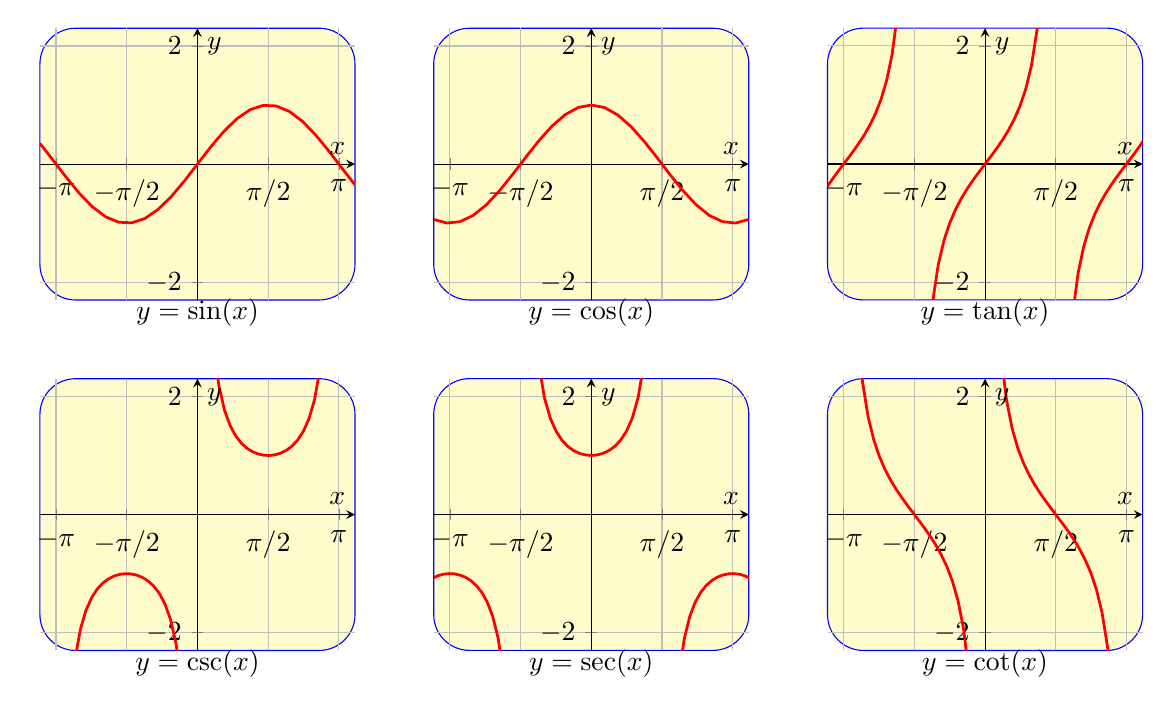
\begin{tikzpicture}
  \begin{groupplot}[
      group style={
          group name=my plots,
          group size=3 by 2,
        },
      width=.33\textwidth,
    ]
    \nextgroupplot[title={$y=\sin(x)$}]
      \addplot[timtam]expression[domain=-3.5:3.5]{sin(x)};
    \nextgroupplot[title={$y=\cos(x)$}]
      \addplot[timtam]expression[domain=-3.5:3.5]{cos(x)};
    \nextgroupplot[title={$y=\tan(x)$}]
      \addplot[timtam]expression[domain=-4.5:-1.58]{tan(x)};
      \addplot[timtam]expression[domain=-1.56:1.55]{tan(x)};
      \addplot[timtam]expression[domain=1.58:4.5]{tan(x)};
    \nextgroupplot[title={$y=\csc(x)$}]
      \addplot[timtam]expression[domain=-3.5:-3.2]{1/sin(x)};
      \addplot[timtam]expression[domain=-3.1:-0.1]{1/sin(x)};
      \addplot[timtam]expression[domain=0.1:3.1]{1/sin(x)};
      \addplot[timtam]expression[domain=3.2:4.5]{1/sin(x)};
    \nextgroupplot[title={$y=\sec(x)$}]
      \addplot[timtam]expression[domain=-4.5:-1.58]{1/cos(x)};
      \addplot[timtam]expression[domain=-1.56:1.56]{1/cos(x)};
      \addplot[timtam]expression[domain=1.58:4.5]{1/cos(x)};
    \nextgroupplot[title={$y=\cot(x)$}]
      \addplot[timtam]expression[domain=-3.5:-3.2]{cot(x)};
      \addplot[timtam]expression[domain=-3.1:-0.1]{cot(x)};
      \addplot[timtam]expression[domain=0.1:3.1]{cot(x)};
      \addplot[timtam]expression[domain=3.2:4.5]{cot(x)};
  \end{groupplot}
\end{tikzpicture}
\end{document}
